\documentclass{beamer}

\usepackage{préambule}
\usetikzlibrary{calc,positioning}

% Morceau d'une ellipse.
% Exemple : \draw (0,0) [partial ellipse=30:150:3cm and 2cm];
\tikzset{
    partial ellipse/.style args={#1:#2:#3}{
        insert path={+ (#1:#3) arc (#1:#2:#3)}
    }
}

\begin{document}

\begin{frame}
	Étant donné une feuille de longueur $L$ et de largeur $l$, comment faut-il l'enrouler pour obtenir un cylindre de volume maximal ?

	\pause

	\begin{center}
		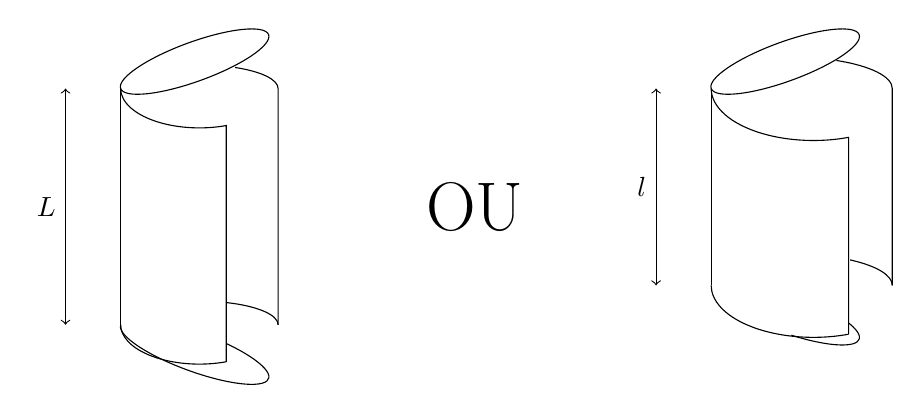
\begin{tikzpicture}
			% Top and bottom
			\draw[<->] (2.3,0) -- node[midway,left] {$L$} ++(0,-3);
			\draw[rotate around={20:(3,0)}] (4,0) ellipse (1 and 0.25);
			\draw[rotate around={-20:(3,-3)}] (4,-3) [partial ellipse=70:-180:1 and 0.25];

			\draw (4,0) [partial ellipse=63:0:1 and 0.3] -- ++(0,-3);
			\draw (4,-3) [partial ellipse=70:0:1 and 0.3];
			\draw (4,0) [partial ellipse=-180:-70:1 and 0.5] -- ++(0,-3);
			\draw (4,-3) [partial ellipse=-70:-180:1 and 0.5];
			\draw (3,0) -- ++(0,-3);

			\node at (7.5,-1.5) {{\Huge OU}};

			% Top and bottom
			\draw[<->] (9.8,0) -- node[midway,left] {$l$} ++(0,-2.5);
			\draw[rotate around={20:(10.5,0)}] (11.5,0) ellipse (1 and 0.25);
			\draw[rotate around={-20:(10.5,-2.5)}] (11.5,-2.5) [partial ellipse=36:-80:1 and 0.25];

			\draw (11.5,0) [partial ellipse=63:0:1.3 and 0.4] -- ++(0,-2.5);
			\draw (11.5,-2.5) [partial ellipse=54:0:1.3 and 0.4];
			\draw (11.8,0) [partial ellipse=-180:-70:1.3 and 0.66] -- ++(0,-2.5);
			\draw (11.8,-2.5) [partial ellipse=-70:-180:1.3 and 0.66];
			\draw (10.5,0) -- ++(0,-2.5);
		\end{tikzpicture}
	\end{center}
\end{frame}

\begin{frame}
	Étant donné deux nombres $a$ et $b$, comment obtenir la plus grande aire possible :\vspace{2em}

	\begin{minipage}{0.47\linewidth}
		\begin{center}
			En construisant un carré de côté $a$ et un carré de côté $b$ ?

			\begin{tikzpicture}[scale=0.7]
				\draw (0,0) -- node[midway,below] {$a$} (2,0) -- (2,2) -- (0,2) -- cycle;

				\draw (3,0) -- node[midway,below] {$a$} ++(3,0) -- ++(0,3) -- ++(-3,0) -- cycle;
			\end{tikzpicture}
		\end{center}
	\end{minipage}
	\hfill\vrule\hfill
	\begin{minipage}{0.47\linewidth}
		\begin{center}
			En construisant deux rectangles de côtés $a$ et $b$ ?

			\begin{tikzpicture}[scale=0.7]
				\draw (0,0) -- node[midway,below] {$a$} ++(2,0) -- ++(0,3) -- ++(-2,0) -- node[midway,left] {$b$} cycle;

				\draw (3,0) -- node[midway,below] {$a$} ++(2,0) -- ++(0,3) -- ++(-2,0) -- node[midway,left] {$b$} cycle;
			\end{tikzpicture}
		\end{center}
	\end{minipage}
\end{frame}

\begin{frame}
	Étant donné une feuille A4, comment découper dedans un patron ayant le volume le plus grand possible ?

	\pause

	\begin{center}
		\begin{tikzpicture}[scale=0.2]
			\draw (0,0) -- ++(21,0) -- ++(0,29.7) -- ++(-21,0) -- cycle;
		\end{tikzpicture}
	\end{center}
\end{frame}

\end{document}